\documentclass[runningheads]{llncs}
\usepackage[T1]{fontenc}
\usepackage{amsmath,amssymb,mathtools}
\usepackage{booktabs}
\usepackage{graphicx}
\usepackage{tikz}
\usetikzlibrary{arrows.meta,positioning}
\usepackage{hyperref}
\usepackage{listings}
\usepackage{microtype}
\usepackage{xcolor}

\newif\ifanonymous
\anonymoustrue

\newcommand{\Rocq}{Rocq}
\newcommand{\coqin}[1]{\texttt{#1}}
\newcommand{\PG}{\mathrm{PGL}(2,7)}
\newcommand{\Unif}{U_G}
\newcommand{\wordlaw}{\mu^{*L}}

\title{Algebraic Specification of Card-Based Cryptographic Protocols in Rocq}
\ifanonymous
  \author{Anonymous}
  \institute{Submission to WADT 2026}
\else
  \author{Cheng-Hui Weng}
  \institute{Nagoya University}
\fi

\begin{document}
\maketitle

\begin{abstract}
Card-based protocols use physical cards to compute with
information-theoretic security. Existing proofs and verification methods do
not combine reusable group-action structure, privacy of executed traces, and
checked finite-step mixing for a concrete protocol. I define a \Rocq{}
framework that treats a finite group, its permutation action, and its shuffle
law as first-class parameters. The main instance uses the action of
$\PG$ on eight projective points. Under an exact uniform shuffle, the
instance has exact correctness, recovery parameters $(t,r,n)=(3,7,8)$, and
view and executed-trace privacy for coalitions of at most three players. These
privacy theorems assume a uniform Boolean secret, a fixed encoded
representative, and passive adversaries. The verifier learns the secret.
Active security, security after the reveal, and composition lie outside the
model. For a finite implementation, I analyze a uniform word of length 200
over five generator letters. A checked fiber-counting certificate proves that
the resulting shuffle law is within unhalved $L_1$ distance $2^{-40}$ of the
uniform group law. This finite-step theorem transfers to single-card
marginals and to a product with any secret prior. It does not establish
approximate coalition-view or executed-trace privacy. Four sibling instances
show which algebraic, operational, privacy, and mixing arguments the framework
reuses.
\end{abstract}

\section{Introduction}\label{sec:introduction}

Card-based cryptography uses face-down physical cards to compute functions
without computational assumptions. A shuffle hides a permutation, while a
reveal exposes selected card faces. Information-theoretic security requires
the resulting observation law to hide the protected secret. Den Boer's
five-card protocol began this line of work~\cite{denBoer1989}. Later protocols
reduced card counts and broadened the class of supported
computations~\cite{MizukiSone2009,MizukiSone2012,KochWalzerHartel2015}.

Mechanized analysis must connect the physical operations to their probability
laws. Koch, Schrempp, and Kirsten use software bounded model checking to
search finite protocol spaces and check lower bounds~\cite{Koch2019}. Their
method gives strong automation for a bounded state space. The development in
this article instead uses a proof assistant to state reusable group actions,
dealer laws, participant views, and executed traces. The target combination
is a group-parametric model with exact trace privacy and a checked
finite-step mixing bound.

The accepted workshop abstract illustrated this algebraic direction with den
Boer's protocol and an $S_5$ development. It also identified Barrington's
theorem as a route from bounded-width branching programs to card
protocols~\cite{Barrington1989,DvorakKoucky2021}. The later $\PG$ instance
now supplies the main case study. Barrington compilation remains future work
and is not a result reported here.

I make three technical contributions.
\begin{itemize}
\item I give a common \Rocq{} interface for a finite group, its permutation
  action, the shuffle law, reconstruction, participant views, and executed
  traces.
\item I prove correctness, the recovery ramp, coalition-view privacy, and
  executed-trace secrecy for the $\PG$ instance under an exact uniform
  shuffle.
\item I prove an unhalved $L_1$ bound between a 200-letter generator-word law
  and the uniform group law. The proof also transfers the bound to card
  endpoints and secret-prior product laws.
\end{itemize}

The exact and finite-step results concern two distinct laws. Exact privacy
uses a uniform group element with a uniform Boolean secret and a fixed dealt
representative. Finite-step mixing compares the generator-word law with that
uniform group law. The current formalization stops at distributional
proximity. It does not transport the bound through the protocol interpreter
to approximate view or trace privacy. The protocol is dealer-based and has no
private inputs. Adversaries are passive. The verifier receives all endpoints
and learns the secret. Active deviations, post-reveal security, and
composition across executions remain outside the model.

Section~\ref{sec:model} fixes the two laws and the security scope.
Section~\ref{sec:framework} presents the framework components used by the
proofs. Sections~\ref{sec:pgl} and~\ref{sec:exact} give the $\PG$
construction and its exact results. Section~\ref{sec:mixing} proves the
finite-step bound. Sections~\ref{sec:instances}--\ref{sec:related} compare
instances, report the methodology, and place the results among related work.
Section~\ref{sec:conclusion} states the remaining bridge and other future
directions.

\section{Protocol and Security Model}\label{sec:model}

The framework describes a protocol by the data
\begin{equation}
  (G,\rho,\mu;R), \qquad U_G, \qquad \mu^{*L}.
  \label{eq:model-data}
\end{equation}
Here $G$ is a finite shuffle group. The representation
$\rho:G\to S_n$ acts on $n$ card positions. The law $\mu$ selects one
generator letter, and $R$ is the real closed field used for probabilities.
The law $U_G$ is uniform on $G$. The convolution $\mu^{*L}$ is the law of the
group element obtained by evaluating $L$ independent letters.

A dealer samples a secret $S$ and a valid dealt arrangement $D$. The action
of a sampled shuffle $g$ produces the arrangement $\rho(g)D$. Player $i$
observes a view $V_i$ derived from the card at position $i$. A coalition
$C\subseteq\{0,\ldots,n-1\}$ observes the joint view
\begin{equation}
  V_C=(V_i)_{i\in C}.
  \label{eq:coalition-view}
\end{equation}
The interpreter executes the dealer, player, and verifier processes. It
records each value received by a process. The resulting record is the
executed trace $T_i$, and $T_C=(T_i)_{i\in C}$ is the coalition trace. The
verifier receives all endpoints and applies the decoder. It therefore learns
$S$ by design.

The primary exact law samples a uniform Boolean secret and uses one fixed
representative $D_s$ for each secret $s$. It then samples an independent
element $g\leftarrow U_G$. For the $\PG$ instance, this is the formal law
named in the source as \coqin{pgl27P}. The representative is the formal orbit
encoder.
\footnote{The exact source objects are \coqin{pgl27P} and
\coqin{orbit\_encode}.}
The all-decks law instead samples a uniform valid arrangement in the selected
secret class before it samples $g\leftarrow U_G$.
\footnote{The robustness law is \coqin{pgl27P\_alldecks}.}
Both exact execution laws use a uniform Boolean prior.

The security theorems concern passive, honest-but-curious adversaries. A
corrupted player follows the protocol and retains its view and executed
trace. Exact coalition privacy states that $S$ and $V_C$ are independent.
Exact trace privacy states
\begin{equation}
  H(S\mid T_C)=H(S).
  \label{eq:trace-privacy}
\end{equation}
The PGL protocol has no private player inputs. Active deviation, security
after the verifier's reveal, and composition across executions are outside
the model.

The finite-step model replaces $U_G$ by $\mu^{*L}$. I measure two laws $P$
and $Q$ by the unhalved $L_1$ distance
\begin{equation}
  \lVert P-Q\rVert_1=\sum_x\lvert P(x)-Q(x)\rvert.
  \label{eq:l1-definition}
\end{equation}
The repository calls Equation~\ref{eq:l1-definition} variation distance.
The common halved total variation distance is
\begin{equation}
  d_{\mathrm{TV}}(P,Q)=\tfrac12\lVert P-Q\rVert_1.
  \label{eq:tv-definition}
\end{equation}
Thus an $L_1$ bound of $2^{-40}$ gives a halved total variation bound of
$2^{-41}$.

Figure~\ref{fig:models} separates the proved paths for the two laws. The
lower path reaches endpoint and product-law proximity. It does not reach an
approximate security statement.
\begin{figure}[t]
  \centering
  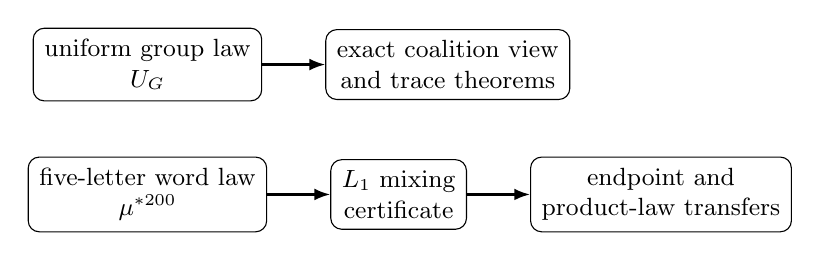
\begin{tikzpicture}[
      node distance=7mm and 8mm,
      box/.style={draw,rounded corners,align=center,inner sep=4pt,
                  font=\small},
      arr/.style={-{Latex[length=2mm]},thick}]
    \node[box] (uniform) {uniform group law\\$U_G$};
    \node[box,right=of uniform] (exact) {exact coalition view\\and trace theorems};
    \draw[arr] (uniform) -- (exact);

    \node[box,below=of uniform] (word) {five-letter word law\\$\mu^{*200}$};
    \node[box,right=of word] (lone) {$L_1$ mixing\\certificate};
    \node[box,right=of lone] (transfer) {endpoint and\\product-law transfers};
    \draw[arr] (word) -- (lone);
    \draw[arr] (lone) -- (transfer);
  \end{tikzpicture}
  \caption{The exact and finite-step proof paths. A transfer from the lower
  path to approximate coalition-view or trace privacy remains future work.}
  \label{fig:models}
\end{figure}

\section{Framework and Generic Theorems}\label{sec:framework}

The group interface fixes the finite carrier $G$, the subgroup of allowed
shuffles, and the permutation representation $\rho$. The interface also
records the generator tuple used by word evaluation. Mathematical Components
provides the finite-group and action structures~\cite{MathComp}. The protocol
instance supplies proofs that the generators belong to $G$ and that the
action preserves valid arrangements.

The sharing interface packages an encoder, a validity predicate, and a full
decoder. Its correctness condition says that decoding a valid encoded
arrangement returns the secret. Its permutation condition says that an
allowed shuffle does not change the decoded secret. The threshold record
stores a privacy cutoff and a decoder that reads the full arrangement. It
does not store a separate recovery threshold. For the PGL instance, the
record therefore packages privacy through three cards and an eight-endpoint
decoder. Section~\ref{sec:exact} proves the seven-card recovery fact outside
that record.

The operational layer represents the dealer, players, and verifier as
processes. Its interpreter executes sends and receives and records process
inputs. An endpoint projection extracts the verifier's final sequence. This
layer connects an algebraic arrangement with the values that processes
receive during a concrete run. It extends the trace-based interpreter from
earlier work~\cite{WengEtAl2025}.

The generic privacy theorem turns transitivity into view independence. Let
$G$ act $k$-transitively on the card positions. If $C$ has at most $k$
positions, then the coalition view under a uniform element of $G$ is
independent of the dealt secret. The theorem applies to any valid encoder
that the action preserves. For the main instance, $k=3$.

The trace theorem carries view independence to execution. Suppose the
interpreter's trace $T_C$ is a function of the mathematical view $V_C$. If
$S$ and $V_C$ are independent, then
\begin{equation}
  H(S\mid T_C)=H(S).
  \label{eq:view-to-trace}
\end{equation}
This theorem separates the probabilistic argument from evaluation of the
interpreter. Each instance proves that its recorded trace equals the expected
view, then applies Equation~\ref{eq:view-to-trace}.

The weighted-word layer defines a distribution on generator letters and
pushes the product law on words through group multiplication. It also maps a
shuffle law to the distribution of each card endpoint. These definitions
allow a group-level $L_1$ bound to pass to endpoints by data processing.

Three small records package results for reuse. A monodromy profile combines a
protocol interface, an endpoint-security witness, and a reconstruction plug.
The witness stores a word law and an endpoint bound. The plug connects the
sharing decoder to the group action.
\footnote{The source records are \coqin{MonodromyProfile},
\coqin{SecurityWitness}, and \coqin{ReconPlug}.}
They organize instance data. The PGL proof chain below uses the underlying
group, sharing, trace, and weighted-word theorems directly.

\section{The \texorpdfstring{$\PG$}{PGL(2,7)} Construction}\label{sec:pgl}

\section{Correctness, Recovery, and Exact-Shuffle Privacy}\label{sec:exact}

\section{Finite-Step Approximation of the Exact Model}\label{sec:mixing}

\section{Other Instances}\label{sec:instances}

\section{Methodology and Artifact}\label{sec:method}

\section{Related Work}\label{sec:related}

\section{Conclusion and Future Work}\label{sec:conclusion}

\subsubsection*{Acknowledgements and AI-use statement.}

\subsubsection*{Disclosure of Interests.}

\subsubsection*{Artifact availability.}

\bibliographystyle{splncs04}
\bibliography{references}
\end{document}
